\documentclass[a4paper,12pt]{article}

\usepackage{geometry}
\usepackage{titling}
\usepackage{titlesec}
\usepackage[english]{babel}
\usepackage[hidelinks]{hyperref}
\usepackage{listings}
\usepackage{xcolor}
\usepackage{graphicx}
\usepackage[export]{adjustbox}
\usepackage{forest}
\usepackage{tikz-qtree}
\usepackage{bchart}

\definecolor{codegreen}{rgb}{0,0.6,0}
\definecolor{codegray}{rgb}{0.5,0.5,0.5}
\definecolor{codepurple}{rgb}{0.58,0,0.82}
\definecolor{backcolour}{rgb}{0.95,0.95,0.92}

\lstdefinestyle{mystyle}{
    backgroundcolor=\color{backcolour},   
    commentstyle=\color{codegreen},
    keywordstyle=\color{magenta},
    numberstyle=\tiny\color{codegray},
    stringstyle=\color{codepurple},
    basicstyle=\ttfamily\footnotesize,
    breakatwhitespace=false,         
    breaklines=true,                 
    captionpos=b,                    
    keepspaces=true,                 
    numbers=left,                    
    numbersep=5pt,                  
    showspaces=false,                
    showstringspaces=false,
    showtabs=false,                  
    tabsize=8
}


\lstset{style=mystyle}

\tikzstyle{startstop} = [rectangle, rounded corners, minimum width=3cm, minimum height=1cm,text centered, draw=black, fill=red!30]
\tikzstyle{io} = [trapezium, trapezium left angle=70, trapezium right angle=110, minimum width=0cm, minimum height=1cm, text centered, draw=black, fill=blue!30]
\tikzstyle{process} = [rectangle, minimum width=3cm, minimum height=1cm, text centered, draw=black, fill=orange!30]
\tikzstyle{subroutine} = [rectangle, minimum width=3cm, minimum height=1cm, text centered, draw=black, fill=yellow!30, double distance=1]
\tikzstyle{decision} = [diamond, minimum width=3cm, minimum height=1cm, text centered, draw=black, fill=green!30]
\tikzstyle{arrow} = [thick,->,>=stealth]

\titleformat{\section}
{\Huge}
{}
{0em}
{}[\titlerule]
\geometry{
	a4paper,
	total={170mm,257mm},
	left=20mm,
	right=20mm,
}

\author{Lucas Standen}
\title{The solution to bad code}

\begin{document}
\maketitle
\newpage
\tableofcontents
\newpage

\setlength{\parskip}{1em}
{\setlength{\parindent}{0cm}

\section{A breif head note and introduction}
This document has been written for the use within AQA computer science 
Alevel coursework. It is published under the MiT license, which I hope
will make it of use to someone other than myself some day on the in's
and out's of simpler compiler design and programming languages as a
whole.

This is the second version of this document, it was writen in GNU
roff before, however I decided to move over to latex for the
more moddern features (notably image support). The latex source for
this document is also avalible along with all referenced code at 
\url{https://github.com/standenboy/school}

Any questions relating to this document should be sent to 
\href{mailto:thing1@seacrossedlovers.xyz}{thing1@seacrossedlovers.xyz}

\section{Analysis}
\subsection{The current problem}
For general small and simple projects, I write in C. However this leads to
hours of debugging due to segfaults, and memory leaks. Due to the languages 
manual memory management the programmer is required to know so much 
information about the hardware they write for, and the second anything goes
wrong, it is vague on how to fix things.

\textbf{I need a language that stops me from shooting myself in the foot}

C has been standard for many decades now and its age is showing, it lacks
many modern features like OOP, or higher level functional abstractions, 
that have become common in modern years due to there helpfulness. This is 
not to fault C's achievements either, the language is my personal choice for
most projects for a reason, it's fast and powerful; any solution I make
should not cut that away.

\subsection{A solution}

\textbf{\textit{Zippy LANG}}

A next generation language, for general use. Designed for keeping code simple,
neat and readable. It will be similar to functional languages, known for 
there strict ability to keep code safe and practical. The language should 
be compiled like C/C++, Haskell and Rust for fast runtime speeds

The goal of Zippy is to make codding easier, while not limiting projects; to 
achive this the compiler will most likely want to use some form of middle man
language to achieve compatibility with more libraries.

\subsection{What is a programming language}
\subsubsection{A very simple explanation}
At its lowest definition a PL is a set of specific words, that when given
to a computer in the right order have a reproducible behaviour. A more human 
way of saying that, would be "It's how we control computers".
\subsubsection{Why are there so many}
When someone is looking at code it can often be seen as just that, however
there are hundreds of languages that all take the idea of "code" in very 
different ways. Some are designed for specific hardware, some are designed 
for making general use programs while others are highly specialized.
It is important to see "code", as more than just one overarching term and
instead see where the code is being used, and evaluate it from that.

\subsection{Researching and getting a scope of the project}
Before I start to design a language i should first find examples of others
and find what i want my language to be like. I'd like my language to feel modern 
so i should take inspiration from what other modern languages do, however on the 
backed i want my language to be  stable and fast, for that i should look at 
older projects.

\subsubsection{Examples of older similar projects}
\begin{description}
	\item[Python] 
		Python is a high level OOP language that was designed in 
		1991. It was made to make programming easy while still being able 
		to use some of C's functions. Although it has become standard for 
		many use cases, it is slow and inefficient, and very bloated.

		\url{https://www.python.org/}

		Zippy should take pythons high level abstractions, as they make 
		programming very easy and it should try and take notes from its 
		libraries as they are mostly well written,
		and well documented.
	\item[Lisp] 
		Lisp is the second ever programming language, developed at MiT, 
		and it is the first functional language, creating many common features 
		like higher order functions, recursion, and garbage collection. It is
		generally not used any more as it feels old compared to other functional
		languages, like Ocaml or Haskell.

		\url{https://lisp-lang.org/}

		Zippy should try to take alot from the syntax of lisp, () make 
		it easy to see what parts of code will effect what, and make 
		things easy to tokenize.
	\item[Perl] 
		Perl is scripting language designed for use in linux, when bash is 
		too slow, or not suited for the job. Perl is often described as the glue 
		of the universe (see xkcd \url{https://3d.xkcd.com/224/}. Its syntax is 
		quite strange however and it is slow. Making it poorly suited towards 
		general use.

		\url{https://www.perl.org/}

		Zippy should take from perls minimalism, it is a small language that is 
		of a similar size to bash or zsh, while feeling closer to python. 
		If Zippy can achieve a similar small size, while remaining
		powerful I will be happy with this outcome.
\end{description}
\subsubsection{Examples of newer similar projects}
\begin{description}
	\item[Gleam] 
		Gleam is a modern language releasing in the past 5 years. It is 
		highly functional, with no mutable data, no traditional loops. 
		Instead recursion can be used to replace alot of these features.
		Gleam compiles to erlang/Beam bytecode, much like java to the
		jvm, and doing this has made Gleam a highly scalable language with 
		good library support out the box.
	
		\url{https://gleam.run/}

		Zippy should take from the functional elements of Gleam, as they keep 
		programs safer, however Zippy should not remove all procedural 
		elements, as for loops are very helpful
	\item[Haskell] 
		Haskell is another modern functional language known for being
		very complicated, however incredibly powerful. Its syntax feels very 
		mathematical, and incredibly terse.

		\url{https://www.haskell.org/}

		Perhaps Zippy could learn from Haskell, as it provides functional and
		procedural elements, making it a well rounded language
	\item[Hare] 
		Hare was designed to be a 100 year language, and thus stability is 
		its main goal, it is not set to
		have a syntax change any time soon, and it has strong emphasis on 
		memory managment like C. It fits into the same part of the tech stack 
		as C, and thus it can be used for some very low level work.

		\url{https://harelang.org/}

		I think Zippy should have a strong emphasis on stability, much like Hare,
		too many times have I segfaulted due to a tiny mistake. Zippy should 
		also look to Hare's small size, you can buy a copy of Hare on a

		\textbf{SINGLE 3 1/2" FLOLPY}

		This is something I too should try to achieve.
\end{description}
\subsubsection{What should be taken away from these languages}
I was already leaning towards functional programming when I started this project however 
now I believe it's the only option for producing safe applications. Zippy will be
a functional language.

I also believe that I should take size of the compiler into account, as this is important 
for keeping the project manageable and maintanable.

And finally I think that syntax should be inspired by Lisp, although Lisp itself can be 
a messy language, with the right changes I am confident that I can make a attractive
language for the 21st century.

\subsection{Clients}
In a project of this nature, the Client is every programmer alive; which is a pretty 
large scope. To narrow this down as much as possible, I will interview a small handful
of people throughout the project, of different skill levels to get a good picture of
what people think of the project.
\subsubsection{Client 1: Amy C}
My first client is a friend of mine, Amy C, she is a confident programmer who has 
completed many complicated projects. I am choosing her as a client as she can give me
technical feed back on my project and its function/utility.
\subsubsection{Client 2: Rayn M}
Another friend of mine, Rayn M, is a technical computer user, however he does not know 
how to program at a high level. He will be a good client as he can show me how my
language looks to some one who doesn't understand the inside workings, helping me 
design the structure of the code to something useable for more people.
\subsubsection{Client 3: Myself}
I've wanted to take out a project like this for a long long time, and this is the 
perfect opportunity to do so, I will be assessing myself along the way of  this, 
building the project to my personal specification.

\subsection{Questionnaires}
It is important to get feedback from end users, so I will take multiple questionnaires 
throughout the project. I will then use them to slightly edit the requirements of my
project this should make the final outcome more helpful and what people want.
\subsubsection{Amy C, initial ideas}
\begin{description}
	\item[What do you find the most important in a language?]
		Speed, readability, debugging ease and disk space efficiency.
	\item[What tools are important for a language to have?] 
		IDE integration (things like tab complete and debugging tools), a 
		package manager, and the ability to interact with the user through the 
		command line easily.
	\item[What features do you like from other languages?] 
		The ability to pass the memory reference of an object or function and a
		collection of built-in or standard functions like "print", "split", 
		or "sort".
	\item[What do you want to program in this language?]
		Lightweight command line tools and web back ends.
	\item[Do you intend to use graphics in the programs you write?]
		Yes.
	\item[Would you prefer a language that focuses on ease of 
		use, or power of code?]
		I like a good balance between the two.
	\item[What were your last 3 projects?]
		A website, a small command-line tool and a midi keyboard (program runs 
		on a Raspberry Pi Pico).
	\item[How many languages would you use on a single project?]
		I try to use as little languages in a single project as possible, so i 
		could likely not use it in an existing project.
	\item[Do you care for low level control, or would you prefer 
		high level abstractions?]
		I think low-level control is very important, but high-level abstractions
		are convenient, so a good balance between the two is best.
	\item[Would you be happy to develop libraries for things that aren't 
		already implemented?]
		Potentially if it is simple enough to implement new things.
\end{description}
\subsubsection{Notes from questionnare 1}
Some of the key things that I'm taking away from this first questionnaire, are my 
client/users initial needs and use cases. I think it's clear my language can be of
assistance to my client, Zippy will be a good language for web back ends and 
small command line tools, which my client expressed interested in.

I find the fact my client is worried by executable size interesting, however
I doubt it will be an issue; a ballooning code-base is unlikely as only one 
person is writing the whole project.

I am also taking on the fact that my client wants good command line tools,
so a pkg-manager and bundler should be a priority, perhaps they could be 
written in Zippy after the compiler is done.

\subsection{The first elements of the project}
At this stage I can say that I'm confident in my project and its scope. I
have a goal in mind for
it.

\textbf{The key things to take away from this section are:}

\begin{itemize}
	\item
		Make a high level language with a useable set of features, to
		replace C in many situations.

	\item
		Keep the language readable and easy, with powerful tools available.

	\item
		Ensure the language is well supported with tools like a pkg-manager.
\end{itemize}

\section{Modelling}
In larger projects, when a programmer needs a data structure that the language
they are writing in doesn't provide, they will need to make their own. This can pose a
challenge to some, especially in low level languages which don't provide anything 
out of the box. 

Bellow are a few examples of these data structures that C doesn't already provide,
that I may use in my project.
\subsection{Linked lists}
this is an alternative implementation of a list, where you store some data, and 
the memory address to the next node. Then you can move through the list by reading 
the data then reading the data of the next node, and then repeating until the 
'next' part of the node is empty.

A diagram showing this can be seen here:

\begin{tikzpicture}
	\tikzset{edge from parent/.style={draw,edge from parent path={(\tikzparentnode.south)-- +(0,-8pt)-| (\tikzchildnode)}}}
	\Tree 
	[.ll
		[.data
		]
		[.next
			[.ll
				[.data
				]
				[.next
					[.ll
						[.data
						]
						[.next
						]
					]
				]
			]
		]
	]
\end{tikzpicture}

In C this is easy to implement as you can find a memory address very easily with to 
find where a bit of data is stored in memory (address of). I will need to use a 'struct', 
which is a bit like a class in C (however you can't attach a function to it, nor use 
inheritance). A simple implementation looks like this:

\begin{lstlisting}[language=C++, caption=Linked list example]
typedef struct ll {
        void *data; // the data of the node
        ll *next; // the next node
} ll;
\end{lstlisting}

The pro's of a linked list are the fact that they can have data appended to the start or 
end easily by changing the root node, or the next node.

Linked lists have a few downsides, for example you can't move through them backwards, 
and unless you store it on its own, you cant find the length of it in a fast way.

In my project I would like to use linked list in the AST (see later sections for info), 
and perhaps to store lists in the language.

\subsection{Dictionaries}
A dictionary is a simple data structure that just stores, a bit of data, and a number or 
string to identify it.
A dictionary like a linked list can be implemented with a struct in c like so:
\begin{lstlisting}[language=C++, caption=Dictionary example]
typedef struct dict {
        void *data;
        int id;
} dict;
\end{lstlisting}

In my project I could use this to hold variables and functions which need to be 
checked and looked up, which is very slow when comparing entire strings, but with this
I can compare integer ID's which is much faster.

\subsection{Prototyping harder features}
\subsubsection{Abstract syntax trees (AST's) theory}
In a programming language many abstract data types will be used to allow the code 
to compile and execute, however I think the hardest part of this is an abstract 
syntax tree. This is a data structure that holds the code in an ordered form that 
can be analysed and  executed in a simple way. It is a tree structure, with the top 
node being a root and all lower nodes being things needed to calculate the root. It can 
be used to show mathematical expressions and function calls, but I thing easiest way to 
show it is via a mathematical example.

Take the follow expression for example:

{\Large{\(1 + (10 * (3 - (2 * 4)))\)}}

We know that this is equal to \(-49\)

However for a computer this is far harder to understand. This is because it has no 
understanding of order of operation.

To solve this we use an AST.

When you solve that expression you know to start with 
\((2 * 4)\), then \(3 -\) 
from that, following the rules of BIDMAS to solve.

We can represent the steps as a tree like so:

\begin{tikzpicture}
	\tikzset{edge from parent/.style={draw,edge from parent path={(\tikzparentnode.south)-- +(0,-8pt)-| (\tikzchildnode)}}}
	\Tree 
	[.+
		[.1
		]
		[.*
			[.10
			]
			[.-
				[.3
				]
				[.*
					[.2
					]
					[.4
					]
				]
			]
		]
	]
\end{tikzpicture}
\\
This will evaluate \(1 + (10 * (3 - (2 * 4)))\)

As you can see, you need to evaluate the expression in the most brackets
first, then the next, and so on, working you way up.

You can evaluate code in a similar way, treating each operation (such as +-*/)
as functions, doing the most deeply nested function first, then working up. 
Each expression can be represented in this tree, then to show a whole program you 
can create a list of trees.

\subsubsection{Abstract syntax trees (AST's) practical}
As a prototype i will make a program that can take mathematical expressions and evaluate 
them, and allowing for functions (in the form f(x)). It will do this via AST's.

This prototype takes 173 lines of code, it takes a string as a cmd line argument then 
converts it into an abstract syntax tree, and finally it executes it. This is just a
simple prototype and thus it is small in scope. It can only do simple operators (+-*/) 
and requires literal values to be surrounded by [] so it knows its not another 
expression to evaluate.

\lstinputlisting[language=C++]{../code/proto/AST/ast.c}
\textit{The main loop for the ast code.}

\lstinputlisting[language=C++]{../code/proto/AST/astg.c}
\textit{The execution loop for the ast code.}

\lstinputlisting[language=C++]{../code/proto/AST/astg.h}
\textit{The definition of the ast, and function prototypes.}

Above is the code for the AST, it stores an operation (which is just an integer), and 
it stores a real left and real right value, along side two other nodes. The real values
are integers, this would be the 2 numbers in reference, in the expression. The 2 nodes are a
recursive data structure, much like putting an object of a class inside the definition of that class
itself. They are used to store values that may still be expressions, for example 
(+ [1] (+ [1] [1])) the second part of this expression would be in the "right" 
variable. 

When code is executed I can check if "left", or "right" are NULL and if 
they are I know that I am at the lowest expression that is only literal values.
Then I can execute that node and work my way up the tree.

The exec function will execute the operation, unless there is a deeper node, if there is 
a deeper node, then it executes it, and places the result in the right or left spot 
respectively.

\textbf{Here is an example input and output:}

 ./ast "(+ (- [3] [1]) (- [3] [1]))"

4

{\small Note the [ ] used to tell the program where the literal values are.}

Overall this was a relatively successful prototype, however it isn't fully functional 
as a language but it has fit the design for a prototype.

\textbf{The code for the AST can be found here:
\url{https://github.com/standenboy/school/tree/master/comp/lucas-standen-NEA/code/proto/ast}}

\subsection{Feedback}
From my first Client (Amy C), she said that putting the numbers inside square brackets 
was inconvenient and annoying and it would be better if the numbers were separated
by spaces instead of separate square bracket surrounded literals.

As this is a prototype I won't fix this issue, however in the actual language this is 
a needed feature that I will be implementing.

\subsection{Mixing linked lists and AST's}
Mixing these 2 data structures together you can represents an entire program. A linked 
list of AST's is how Zippy will represent all code the user writes. To do this, use a 
linked list, and in the data element put a AST, then the next node can contain the same. 
This might be a help to zippy as the compiler can convert all code to an AST, then 
compile it.
\section{Objectives}
Zippy must support the following features, it needs them to be a usable language that has 
many uses.
\subsection{Core objectives}
\begin{description}
	\item[A compiler for the Zippy language]
	\item[AST's used to compile source code]
	\item[A lisp like syntax]
	\item[Functional paradigm language]
	\item[Recursion]
	\item[Higher order functions] \textit{(this means functions can be passed as arguments to 
		other functions)}
	\item[High performance language]
	\item[A package manager]
	\item[Ability to call C functions]
\end{description}
If possible I would like Zippy to also meet the following extra objectives. While not needed to make the project
usable, it will make it far nicer to work with.
\subsection{Extra objectives}
\begin{description}
	\item[String parsing in the stdlib]
	\item[graphs in the stdlib]
	\item[networking in the stdlib]
	\item[graphics in the stdlib]
\end{description}

I think with these objectives in mind I will make a well rounded language that achieves my
goal of being used in the same way and places that C is. If all goes to plan I will 
create a high level, compiled, functional programming language.

\section{Design}
\subsection{Language specification}
Like any other programming language Zippy needs to have a defined syntax, bellow
you can find a syntax for zippy that will be complaint with my objectives.
\subsection{Keywords}
\begin{description}
	\item[defun] starts the definition of a function, will take in a name, return type, and arguments with types
	\item[endfun] ends the definition of a function
	\item[let] define a variable with a initial value, takes a variable name and a value
	\item[set] change a pre defined variable, takes a variable name and a new value
	\item[def] define a variable which doesn't have a initial value, takes a variable name
	\item[defunptr] defines a ptr to a function same as defun, but used to pass functions as arguments
	\item[if] starts an if block, takes a condition
	\item[elif] starts an elif block, must come after and if block, takes a condition
	\item[else] starts an else block, must come after an elif or if block
	\item[endif] must be at the end of an if/elif/else block
	\item[for] defines a for loop, takes a variable name to use as an iterator, a starting value for that variable, a condition, and a difference to change the iterator by each loop
	\item[endfor] ends a for block
	\item[symbol] defines a function for semantic purposes from an external executable, take a name and arguments, the symbol must be in a linked binary
	\item[+] addition, takes 2 arguments
	\item[-] subtraction, takes 2 arguments
	\item[*] multiplication, takes 2 arguments
	\item[/] division, takes 2 arguments
	\item[=] equality comparison operation, takes 2 arguments
	\item[!=] negative equality operation, takes 2 arguments
	\item[\(<\)] less than equality operation, takes 2 arguments
	\item[\(>\)] greater than equality operation, takes 2 arguments
	\item[\(<=\)] less than or equal operation, takes 2 arguments
	\item[\(>=\)] greater than or equal operation, takes 2 arguments
	\item[exit] exits the program, takes a value to exit on
	\item[return] returns from a function, and takes a value to return
	\item[alloc] allocates a block of memory, takes a size in bytes
	\item[struct] defines a struct, takes a name as an argument
	\item[endstruct] ends the definition of a struct
	\item[sizeof] returns the size of a given type, takes the type name as an argument
\end{description}  
\subsection{Other code elements}
As one can see from the list of keywords, all blocks such as functions are defined and ended. This leads to a nice
form of code that isn't reliant on indentation, where blocks can be easily seen. I have made sure to keep the 
language uniform, so function, struts, if statements and for loops all use this syntax.

Comments can be written in zippy by prefacing a line with a '/'.

All code must have a main function, if it doesn't the linker will fail. This is the entry point to the program, so
it is where code will start executing from.

Reverse Polish notation is used for mathematical and comparison operations, so \((2 + (4 + 3))\) would be written
as \((+\; 2\; (+\; 4\; 3))\). 
\subsection{Memory management}
In zippy memory is semi manual to manage, like in C the programmer needs to allocate blocks of a large enough size,
however they do not need to free the memory, as all allocs will be freed just before a function returns. This means 
that memory has a life time of the function it was defined in. One should note that this means that if an allocated 
block needs to be returned, the caller function needs to allocate the block, or else the memory returned will be 
freed as soon as the function has finished. 
\subsection{The steps in compiling a zippy program}
All the programmer should need to do is call the "zpy" command, and then the code will be converted from zippy to 
binary. However on the back end of the project, more has to happen. First the zippy code gets converted to C, this 
is how zippy will be cross compatible with C, then the C code is compiled to ASM, then the ASM, is converted to
binary, and finally the linker will convert the binary into an executable, and add any libraries that are used.

For my project I will only need to do the first step, and slightly edit the second step, as C compilers, assemblers
and linkers already exist. So I don't need to reinvent the wheel.
\subsubsection{Converting zippy to C}
The process of converting zippy to C is yet again another long one. It starts with reading in the program, 
then converting that into individual expressions (in zippy one expression takes up one line), then the expression
is converted to a data structure that holds a function name, and its arguments in individual variables and finally
it converts that data structure to C code via substituting names, functions, and literal values into template C code.
\subsection{Actually using zippy}
For the programmer to use zippy they must be able to call it as a command, on a text file containing their code and
they must give an output file name, to place the binary. To call the command, it can be simply done using the command
line with the "zpy" command, which the user will need to install, this is the compiler.

The compiler will have the following options to tweak the output.
All options are prefixed with a '-', to denote that they are not the input file.

\begin{description}
	\item{o} - changes the output file location
	\item{i} - tells the C compiler to include a library that is given after this argument
	\item{c} - tells the zippy compiler to return C code instead of a compiled binary,
		this is helpful when using zippy to make small functions in a C/C++ code
		base
	\item{f} - pass a flag to the C compiler, the next option should be an argument 
		accepted by gcc.
\end{description}

The programmer will also have access to "zpypkg" which will automatically setup their project with compile commands 
and a template executable. It will be a very simple tool, that copies needed files around to the correct folders,
it will be written using Bash, (the main scripting language used by unix, along with sh and perl). It will have the 
following arguments to allow the programmer to quickly write zippy code.

C\begin{description}
	\item[init] this will initialize the package manager, creating the needed files.
	\item[advinit] this is an advanced form of init, it will set things up to have interoperability with C.
	\item[build] this command can be used from within a zippy project directory, and will build the project into an executable.
	\item[run] this will build the project, and run the newly built executable.
	\item[clean] this will remove all temp files and binaries from the project folder, this is helpful when sharing code.
	\item[remove] this will remove zpypkg from the current directory (think of it like a de-init).
\end{description}

\subsection{Modelling the compilation process}
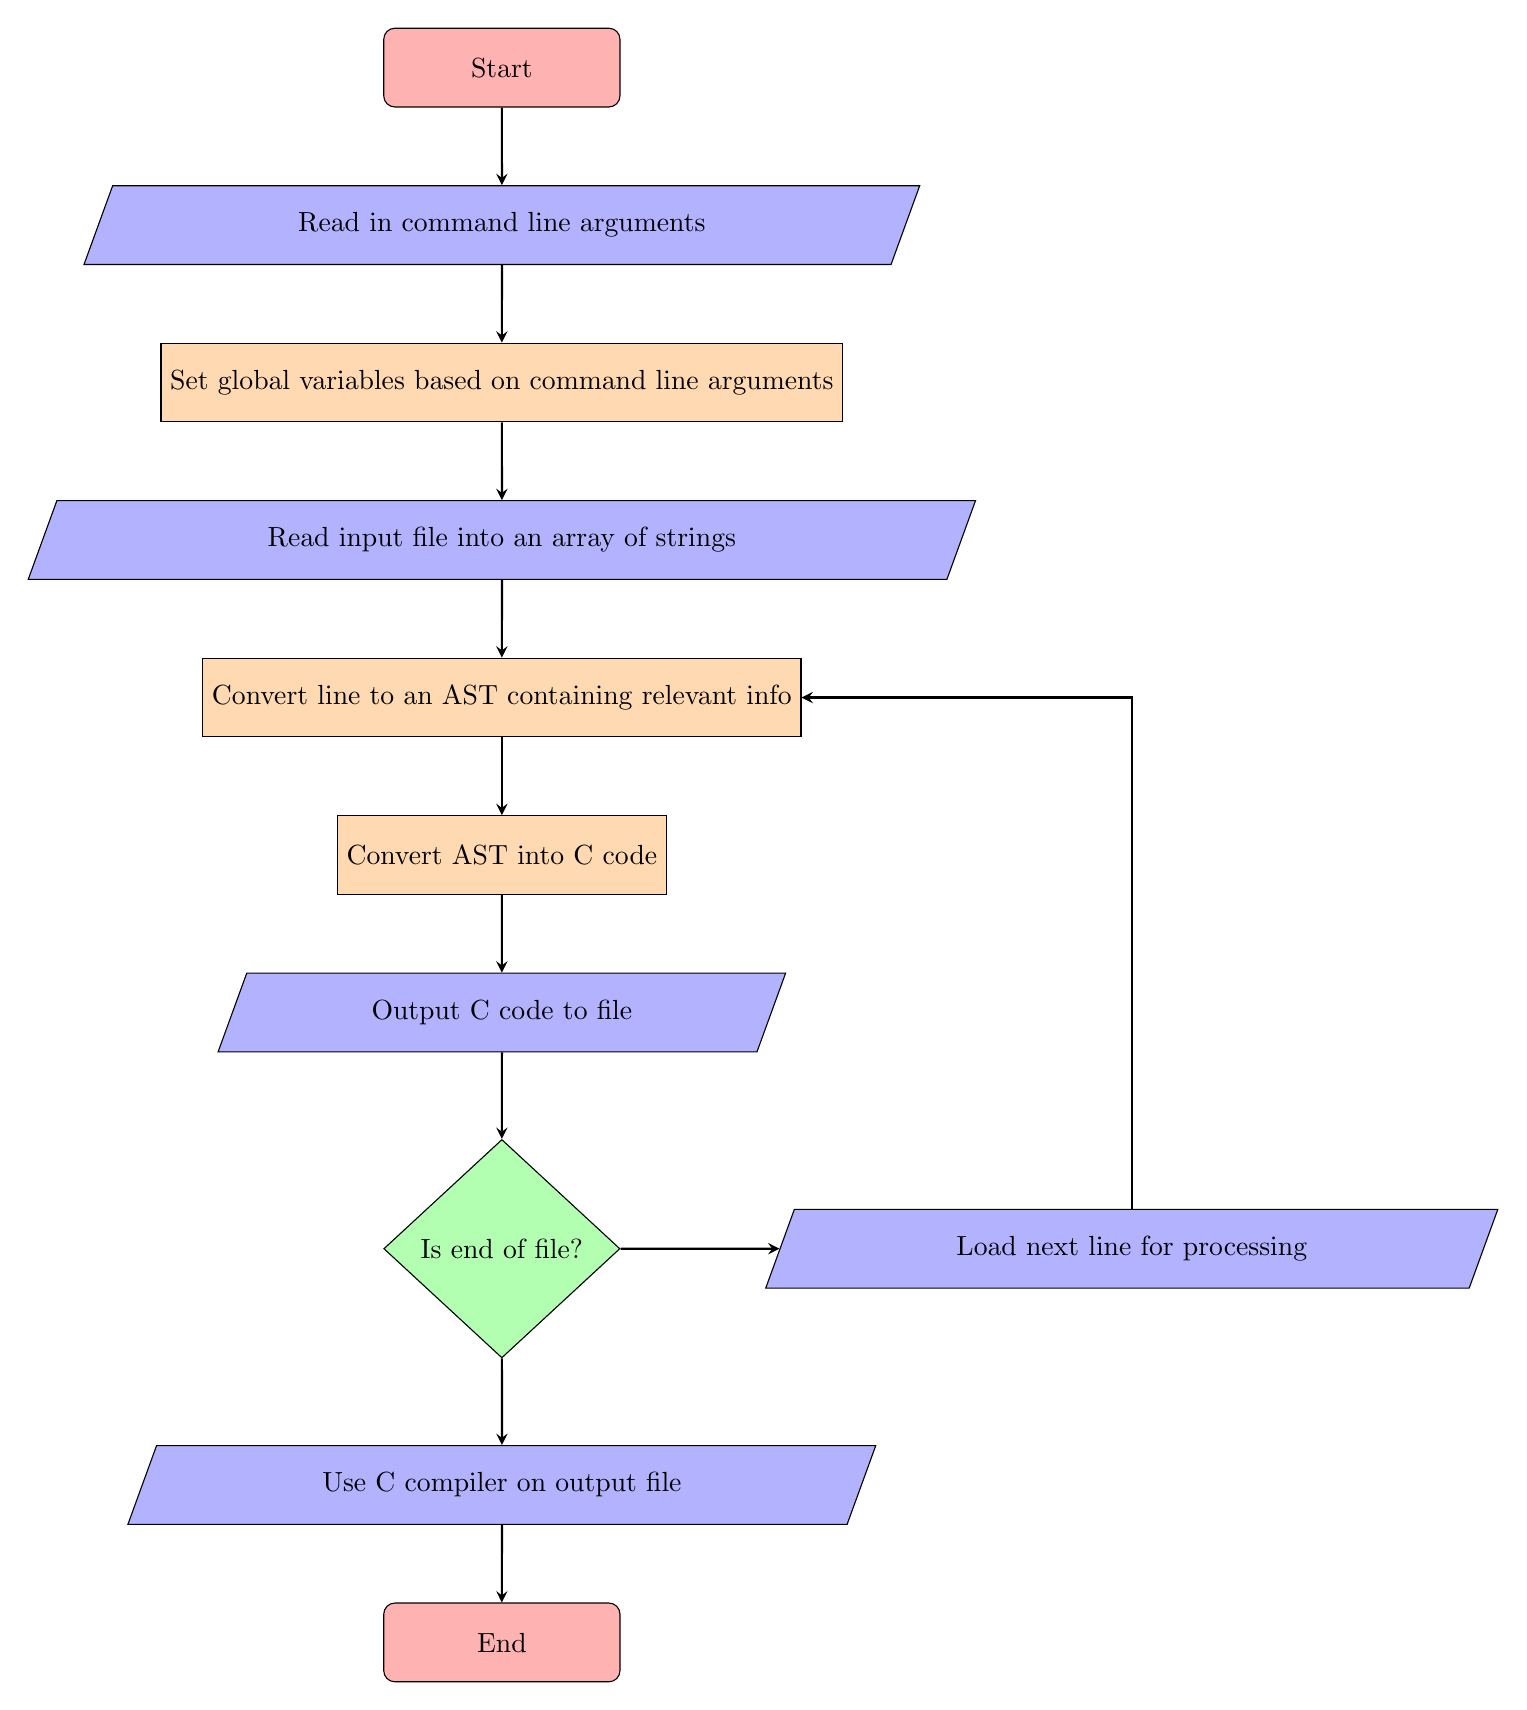
\begin{tikzpicture}[node distance=2cm]
	\node (start) [startstop] {Start};

	\node (in1) [io, below of=start] {Read in command line arguments};
	\node (proc1) [process, below of=in1] {Set global variables based on command line arguments};
	\node (in2) [io, below of=proc1] {Read input file into an array of strings};
	\node (proc2) [process, below of=in2] {Convert line to an AST containing relevant info};
	\node (proc3) [process, below of=proc2] {Convert AST into C code};
	\node (out1) [io, below of=proc3] {Output C code to file};
	\node (dec1) [decision, below of=out1, yshift=-1cm] {Is end of file?};
	\node (proc4) [io, right of=dec1, xshift=6cm] {Load next line for processing};
	\node (out2) [io, below of=dec1, yshift=-1cm] {Use C compiler on output file};

	\node (end) [startstop, below of=out2] {End};
	
	\draw [arrow] (start) -- (in1);
	\draw [arrow] (in1) -- (proc1);
	\draw [arrow] (proc1) -- (in2);
	\draw [arrow] (in2) -- (proc2);
	\draw [arrow] (proc2) -- (proc3);
	\draw [arrow] (proc3) -- (out1);
	\draw [arrow] (out1) -- (dec1);
	\draw [arrow] (dec1) -- (out2);
	\draw [arrow] (out2) -- (end);
	\draw [arrow] (dec1) -- (proc4);
	\draw [arrow] (proc4) |- (proc2);
\end{tikzpicture}
This is a high level diagram of what will go on in my code, with each box corresponding to around 1 function.

\subsection{Modelling data structures I will use}
\subsubsection{AstNode}
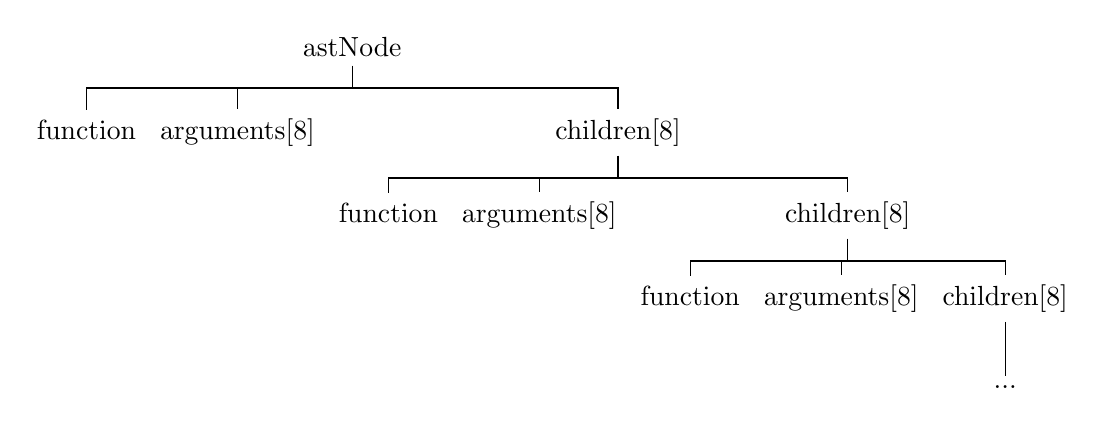
\begin{tikzpicture}
	\tikzset{edge from parent/.style={draw,edge from parent path={(\tikzparentnode.south)-- +(0,-8pt)-| (\tikzchildnode)}}}
	\Tree 
	[.astNode
		[.function
		]
		[.arguments[8]
		]
		[.children[8]
			[.function
			]
			[.arguments[8]
			]
			[.children[8]
				[.function
				]
				[.arguments[8]
				]
				[.children[8]
					[....
					]
				]
			]
		]
	]
\end{tikzpicture}
\\
This is the main data structure that powers the compiler, it takes a fuction name as a string, an array of 8 arguments as
strings, and an array of 8 children as astNodes. The fuction argument will be the first word of a line of Zippy, it is the 
name of the function. The argument variables are each litteral argument, such as a string or integer litteral that is given
to the fuction, this can be empty. The children argument contain more astNode, they are arguments that are given in the 
form of functions, for example (printint (+ 2 2)), would result in (+ 2 2) having its own astNode made, and put as the child
of the (printint) astNode.

\subsubsection{Array list}
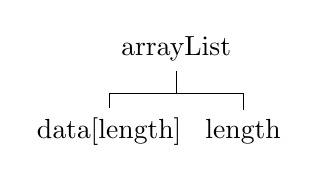
\begin{tikzpicture}
	\tikzset{edge from parent/.style={draw,edge from parent path={(\tikzparentnode.south)-- +(0,-8pt)-| (\tikzchildnode)}}}
	\Tree 
	[.arrayList
		[.data[length]
		]
		[.length
		]
	]
\end{tikzpicture}
\\
This is a far simpler data structure, it is useful in languages such as C, C++ and rust to represent non fixed length
arrays. This is because in these languages arrays are stored as continous bytes in memory, making it hard to tell where
they end. An array list is a data structure that store the array with an interger value of the length, thus making it
so one knows how long the list is. This is important to avoid runtime errors such as segmentation faults, caused by 
reading out of bounds memory.

\subsection{Why so few?}
It was an intentional choice to uses so few data structures, in languages like C, where OOP is not possible,
the importance of bundling data is far smaller, with arrays and variables being far more useful than anything
else; they have faster runtime speeds and a cleaner syntax that makes them preferable. One will find alot of
C projects will follow this phylosophy, as it generally leads to better projects.

\section{Implementation}
As has been previously mentioned, zippy will have its compiler written in C and its package manager writen in bash.
The code will be displayed bellow, it has been commented to use a tool I wrote called autodoc, which can function
like a doc-string in python, after each file I will explain in detail what it does and why it is in its own file.

\lstinputlisting[language=C++]{../code2/zpy.c}
\textit{zpy.c}

This is the main executable, containing my main function, which is the program entry point. This file handles the
opening of input and output files, calling other functions, and processing the command line arguments.
\lstinputlisting[language=C++]{../code2/fileread.c}
\textit{fileread.c}

This file is responsible for reading in the file contents, into and array list of strings (an array list is an array
with a length attached to it, to help with memory managemnt). This file also handles the stripping of tabs and other 
forms of white space.

\lstinputlisting[language=C++]{../code2/tokenizer.c}
\textit{tokenizer.c}

This file has the job of converting a single line of code into An abstract syntax tree, it splits each expression into
its function name, as a string, and each of its arguments (max 8) as a string, and if there are nested function calls, 
it will create more AST nodes for them, in the recursive data structure. The main tokenizer function is using
a lesser known feature of the C programming language, \textit{goto}, it uses this to achieve recursion, without needing
to define a second function, as goto lets the user define a label in their code, just like in ASM. 

\lstinputlisting[language=C++]{../code2/appendsnprintf.c}
\textit{appendsnprintf.c}

This is a smaller file, that defines a helper function used heavily in the comp.c file, this function allows the user
to concatenate an unknown amount of strings together. It uses another lesser known feature of C, \textit{vardic functions},
which allow the program to parse an unknown amount of arguments to a function. This function is needed, as C does not
provide an effective way to concatenate strings multiple times, the function that this is built off \textit{snprintf} can only be used 
once per variable, which didn't fit my use case.

\lstinputlisting[language=C++]{../code2/comp.c}
\textit{comp.c}

This file is by far the largest and most important in the program, it converts a zpy AST to C code, and writes it to an output
file. It also handles syntax errors in the users code. The first function from this file that is called, is the CompilerInit,
this sets up an interrupt which is used to jump the program to a different point, if there is a syntax error.

The next function from this file that is called, is the main Compile function, this is actually a wrapper around the compile function.
This function is used to set the current line, which is used if there is an error, call the main compile function, write to 
the output file and add newlines, if needed. And finally it handles the automatic free function of zippy.

The main function that this provides is the compile function, this starts by processing child arguments, A child argument can be created
by the tokenizer when a nest function is used in zpy, for example (let a:int (+ 2 2)), in this case the child function is (+ 2 2). It
will compile the children function first, using the processChildren function, assigning their outputs to the argument section of the AST.
It then uses a large if block, to determine which function it is needing to generate. Each branch, use the appendsnprintf function to
combine the arguments and templated C code. The checkNULL function is used a lot in this function. This is because if the user does 
not provide enough arguments to a function call, which is the most common syntax error after a missing bracket, the argument slot, will
be null, thus I can check if it is NULL, to tell if the user made an error. If an error is made a signal is sent to the process, which 
will cause the interrupt handler function to be triggered, telling the user the line number they made the error on with a brief description
of the issue.

Also in this file are a handful of helper functions in the conversion process, these convert zippy's reverse polish notation to traditional 
infix definition, and convert zippy's type annotations to C's type annotations.

Finally, as previously mention there is the errorhandle function. This is triggered by a signal being sent to the program, and will cause 
it to stop instantly, and will trigger an error print.

\lstinputlisting[language=C++]{../code2/util.c}
\textit{util.c}

This file defines a smaller helper function, which is used in the main executable to gracefully exit if there is an error.

\subsection{Header files}
\lstinputlisting[language=C++]{../code2/fileread.h}
\textit{fileread.h}
\lstinputlisting[language=C++]{../code2/tokenizer.h}
\textit{tokenizer.h}
\lstinputlisting[language=C++]{../code2/comp.h}
\textit{comp.h}
\lstinputlisting[language=C++]{../code2/appendsnprintf.h}
\textit{appendsnprintf.h}
\lstinputlisting[language=C++]{../code2/util.h}
\textit{util.h}

These files are used internally to allow for the linking of C code to function properly; see the following section for 
more info on the C linking process.

\subsection{The C linking process}
When one writes C code, it is first compiled by a compiler, in most cases this is a compiler like GCC, or clang.
These will convert the C code into ASM, (sometimes through a middle man language to make compiling for many systems
easier), which then gets assembled into an object file. These object files are not executable, in this state they
are libraries that can be used in other code. To make them executable they must be linked with the C stdlib and any
other used binary files; this is done by the linker. The linker will take the list of symbols defined in the object file,
each symbol will correspond to one function in C. It will also take all the symbols in the libarys that the code is linked 
with. This means common libraries only need to be compiled once, and the linker can take pre compiled binarys.

In this project, each .c file is converted to a .o file (an object file), and then the linker will link all of them together
to produce the final executable.

To automate the process of compiling and linking, I've used a make file, a build tool which can have multiple functions defined
that will compile all the given code. Here is makefile:

\lstinputlisting[language=C++]{../code2/Makefile}

This may look confusing, however its goal is very simple, each label (which are denoted with a ':') is a function 
that can be run, the 'all' function is an omni function ran when the user types in 'make' with no arguments, whereas the others 
can be called with 'make install' and 'make clean'. The .c.o label is special, it compiles every C file, to a .o file, this is a 
shorthand syntax, that isn't very readable, but is easy to use. The .PHONY function is another special option, this is used to ensure 
autocomplete works in the terminal when typing the make commands. Finally the variables defined at the top, are used to define compiler
options. In this case, im using -O3, which tells the compiler to perform the maximum optimisations to my code. Ensuring the compiler is
fast.

\subsection{Zpypkg}
To make the package manager, I will be using bash to generate simple build scripts and default files. The tool doesn't need to do too
much it just needs to make it easier to initialize a project. It will not use networking in any way, instead, it will leave it up
to the programmer, so they can use any protocol or tool they like, such as git.

The code for zpypkg can be seen below.
\lstinputlisting[language=Bash]{../code2/zpypkg/zpypkg.sh}
\textit{zpypkg.sh}

This code is very simple, it can create a default main.zpy file and a zpybuild.sh file that can be used to compile a zpy project 
in one instruction. It also has build and run functions to allow the developer to quickly produce and run up to date binaries.

\subsection{Zpylib}
The language needs a simple standard library that will handle the simple IO functions, this is by no means perfect but it is a 
good enough base, that it can be easily extended to a full project.
\lstinputlisting[language=C++]{../code2/stdlib/zpylib.c}
\textit{zpylib.c}

These functions for the most part are a wrapper around the c stdlib, which is what makes them such a good base to use.

\lstinputlisting[language=C++]{../code2/stdlib/String/String.c}
\textit{String.c}

These functions will create a simple object oriented style development for the use of strings, allowing the user to split, create,
destroy and insert into strings. This library allows the user to easily make parsers and other such string related tools.

\subsection{Other libraries}
While I haven't ported or made any other libraries for zpy, this doesn't mean they can't be used, as long as a library can be linked
with C code (see the linking section above for more info), it can be used within zpy, and any function in the C stdlib is already
available to use. I will use this later in my examples to use the raylib graphics library.

\section{Testing}
\subsection{Introduction}
To test zpy, I have made a few sections of example code, to test that the compiler can indeed convert code to C. I decided I would
test the following
\begin{description}
	\item[Recursive Fibonacci program] A simple program that will calculate the n'th Fibonacci number
	\item[String splitting] A small program that splits a string, to test the string processing class
	\item[A incorrect program] To test the languages error messages
	\item[A hello world program using zpypkg] To test that zpypkg can be used to manage projects
	\item[Space invaders] Using the raylib graphics library, I will build a clone of space invaders
\end{description}
\subsection{Fibonacci}
The N'th number in the  Fibonacci sequence can be calculated by adding the previous 2 numbers in the sequence, and assuming the first 
2 numbers are both 1.

For example here is the first few digits:

\(1, 1, 2, 3, 5, 8, 13, 21\)

\subsubsection{Code}
In zpy this code can be written as follows:

\lstinputlisting[language=lisp]{../code2/examples/fib_example.zpy}
\textit{fib\_example.zpy}

A simple explanation of what is happening in this code is,

\begin{description}
	\item[] I make a function called fib, that returns an int, and takes an int called \(n\) in as input
	\item[] I create a base case using the if statement, comparing if \(n < 2\)
	\item[] I return the value of \(n\) if it is less than 2
	\item[] Otherwise I return the sum of the previous to values in the sequence
	
	\item[] I then define a main function that is marked as returning an int, this is where execution of the 
		program begins
	\item[] I prompt the user for an input and read it in as an integer
	\item[] I perform the fib calculation and print the value
\end{description}


\subsubsection{Demo}
\lstinputlisting{./examples/fib.example}

55 is indeed the 10th Fibonacci number. 

The following python code produces the same output

\lstinputlisting[language=python]{./examples/fib.py}
\textit{fib.py}

\subsubsection{Performance}
The zippy code is orders of magnitude faster than the python code, the time command in Unix can be used to show this.

\begin{center}
\small{\textit{A table comparing the performace of zippy and python, when finding the 30'th Fibonacci number.}}
\end{center}
\begin{center}
\begin{bchart}[max=0.4]
	\bcbar[label=Zippy, color=yellow]{0.02}
	\smallskip
	\bcbar[label=Python, color=blue]{0.339}
	\smallskip
	\bcxlabel{time in seconds \textit{lower is better}}
\end{bchart}
\end{center}

\subsection{String splitting}
\subsubsection{Code}
The following code is a simple example of string splitting in zpy, using the standard library. All it does 
is split the string hello\_world into the substrings of hello and world, using the \_ as a delimiter.
\lstinputlisting[language=lisp]{./examples/str_example.zpy}
\textit{str\_example.zpy}

The code is in 3 main sections:
\begin{description}
	\item[] Defining the starting string
	\item[] Splitting the string
	\item[] Cleaning up the memory
\end{description}
\subsubsection{Output}
\lstinputlisting{./examples/string.example}
\subsubsection{Explaining}
The cleaning of the memory isn't strictly needed in this situation, as it will be freed automatically when
the program ends. As Zippy is closely related to C, this is still a needed feature for the program to be 
safe, however code written in Zippy has some extra safety features, such as auto freeing of memory when 
a function finishes. However as that feature only works on memory allocated with \((alloc)\), freeing must be done
manually for other things, such as the string library.

\subsection{zpypkg example}
To use zpypkg I wanted it to be very easy, and hassle free. Other packaging tools like cargo, require entire
projects to be built with them in mind, this forces a specific project structure that isn't tuned to all use
cases. I believe that \(Go\) hits the mark on a good packaging tool, it is clean, small and out of the way, 
simply providing automated builds and running of the code.
\subsubsection{Using zpypkg}
\lstinputlisting[language=bash]{./examples/zpypkg.example}
Its as simple as that! Out of the way, and customizable via the build.sh file that zpypkg generates.

\subsection{Space invaders}
\subsubsection{Background}
To build a small space invaders game, I'm going to use the raylib graphics library 
(\url{https://www.raylib.com/})
based on GLFW. It is well known and over 10 years old at this point, it is fast, supports most devices and 
operating systems under the sun, and is written in C for C, and due to this, it is also compatible with Zippy!
\subsubsection{Code}
\lstinputlisting[language=lisp]{./examples/spaceinvaders.zpy}
\textit{spaceinvaders.zpy}

While this may look like a large amount of code, it is actually quite simple, it opens a window, starts a loop, if
the player shoots the alien it takes damage, if the alien has taken enough damage the game ends, and if the alien 
reaches the ground the player loses. For simplicity's sake, the program uses exit codes to establish what the outcome
of the game was, this can be checked on a Unix like system like so: echo \$?. For this game, if this returns a 0, the
player has one, otherwise the alien enemy has won
\subsubsection{Seeing it go}
Bellow is a screenshot of the game working, its graphics are minimal to say the least, but it does prove Zippy can be 
used with C libraries.

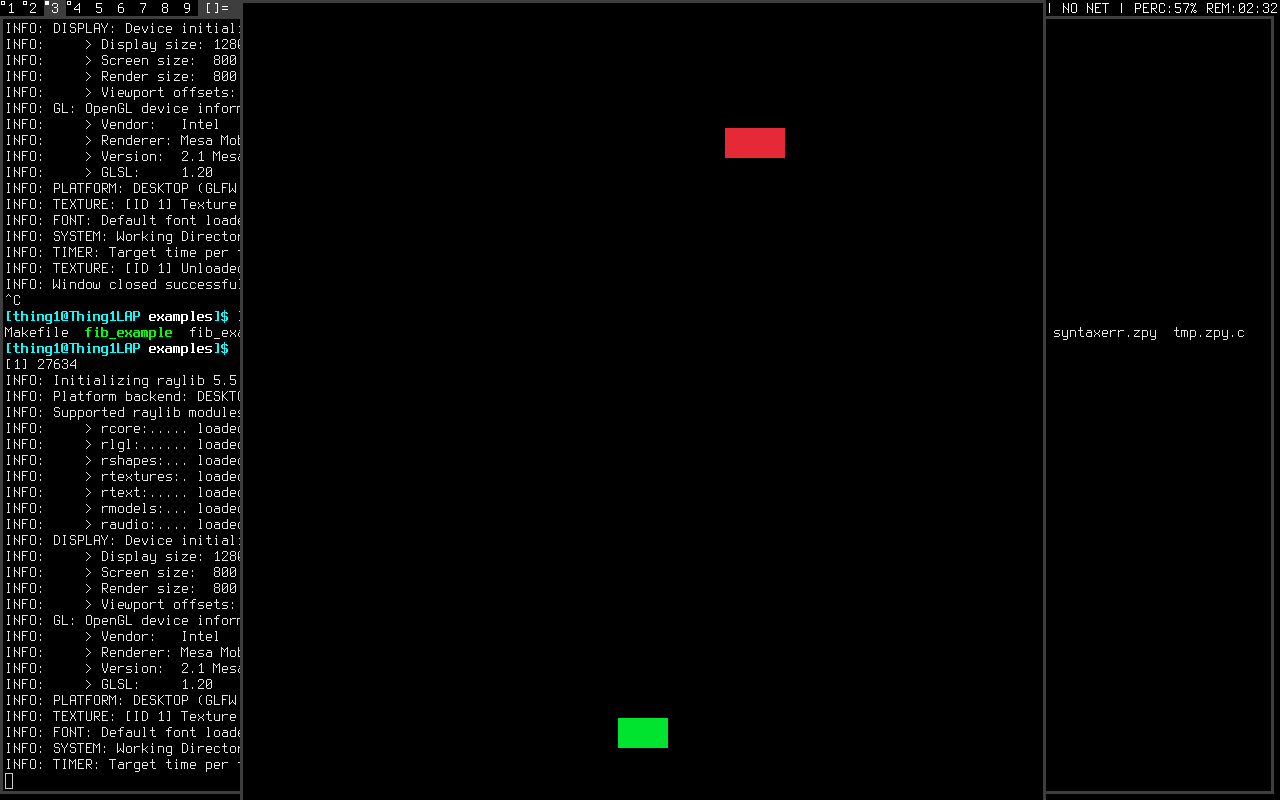
\includegraphics[width=\textwidth, left]{./examples/spaceinvaders.png}
\textit{The player is green, The alien is red}

\section{Evaluation}
At this stage in my project, I have created a full project, and now I need to compare it to my original goals. 

Here is a copy of my original goals to avoid needing to flick between many points.
\subsection{Core objectives}
\begin{description}
	\item[A compiler for the Zippy language]
	\item[AST's used to compile source code]
	\item[A lisp like syntax]
	\item[Functional paradigm language]
	\item[Recursion]
	\item[Higher order functions] \textit{(this means functions can be passed as arguments to 
		other functions)}
	\item[High performance language]
	\item[A package manager]
	\item[Ability to call C functions]
\end{description}
\subsection{Extra objectives}
\begin{description}
	\item[String parsing in the stdlib]
	\item[graphs in the stdlib]
	\item[networking in the stdlib]
	\item[graphics in the stdlib]
\end{description}

\subsection{Comparing the goals to the product}
In order I will evaluate and show where and how these came to be.

\subsubsection{A compiler for the Zippy language}
This was the main goal of the project and I achieved this perfectly as planned, the compiler generates C code that runs
quickly and efficiently with extra safety features. This is a language that is less dangerous that C, while keeping the 
same performance.

This goal was fully met.

\subsubsection{AST's used to compile source code}
This was a goal for the internal design of the project, and I achieved this too with my ast\_node tree data structure, 
it made the rest of the compilation process far easier as there was less worry for passing data around in random ways.

This goal was fully met.

\subsubsection{A lisp like syntax}
This goal was also met thanks to the advanced tokeniser I wrote that is capable of generating AST's from individual lines 
of Zippy, you can see this first hand when you look at the use of parentheses in the language.

This goal was fully met.

\subsubsection{Functional paradigm language}
This goal is more up to argument, as to weather I achieved it or not. The language definitely has many features from functional
programming, however none of them are enforced, making it harder to achieve the benefits. In terms of paradigm I feel Zippy
fell closer to imperative, but one should note Zippy does support all major functional features, such as higher order functions and
recursion. Functional programming really shows its benefits when it is used exclusively, which isn't done in zippy, however with 
determination, one could definitely use Zippy in the same way one uses Lisp.

This goal was met, however not to the fullest.

\subsubsection{Recursion}
As zippy is dependant on C, it can support any feature C can out the box, and C is perfectly capable of using advanced recursive 
algorithms.

This goal was fully met.

\subsubsection{Higher order functions}
To achieve this goal I created the \((defunptr)\) keyword which allows the programmer to pass a function as a pointer from within 
a struct or variable. I find this to be a very elegant way of implementing higher order functions, as it is very simple for 
low level development, which is where Zippy lies on the tech stack.

This goal was fully met.

\subsubsection{A high performance language} 
As it was previously seen in the examples section, zippy has been able to crush python, and for me this was enough. For most 
use cases python is fast enough, and thus zippy being faster means it will never be too slow.

This goal was fully met.

\subsubsection{A package manager} 
I believe zpypkg was exactly what I wanted to make, it is small fast and too the point, it doesn't get in the programmers way
like larger tools available.

This goal was fully met.

\subsubsection{Ability to call C functions}
Zippy is fully able to call C functions and I even created a keyword to define prototypes for them \((symbol)\), this made
it very easy to call C functions when needed, however it is not needed, as the linker is what puts in most the work to
achieve this.

This goal was fully met.

\subsection{Thoughts on the core objectives}
I believe that I have hit all of my core objectives well enough to define my project as complete, I have made a programming 
language that I would happily use for many projects, with it supporting all the features I could need. Although if I had more 
time there are some things I would have liked to add, notable a more full standard library, as of current Zippy is reliant
on the C stdlib and many of its downsides have been passed over into Zippy.

\subsection{Extra objectives}
While these were optional, I still took the liberty of making them to make a more achieved project. I did not complete them
all due to time constraints. I made string parsing and graphics available in the standard library, via the string functions
previously shown, and linking with the raylib graphics library.

One could argue that all of these things are possible, as it is possible to link with a pre existing library to do the work 
for you, but in some ways that cheating, and also won't work for libraries written in c++.

}

\end{document}

